\section{Introduction} \label{sec:introduction}

% Narrow in
\emph{Mesh composition} is the process of assembling several pre-modeled 3D objects into a unified asset.
It is a fundamental part of many 3D content creation workflows, in which an artist selects \emph{accessories} from an existing library and manually rotates, translates and deforms them to fit realistically on a character's \emph{base mesh} without intersections (see \autoref{fig:teaser}).
Automating this tedious task is a critical and challenging research question combining \emph{geometric} and \emph{physical} constraints (the two meshes must be close to each other without intersecting) with \emph{semantic} alignment (e.g., a pair of glasses should sit on the eyes in the correct orientation).



\begin{figure*}
    \centering
    \vspace{3mm}
    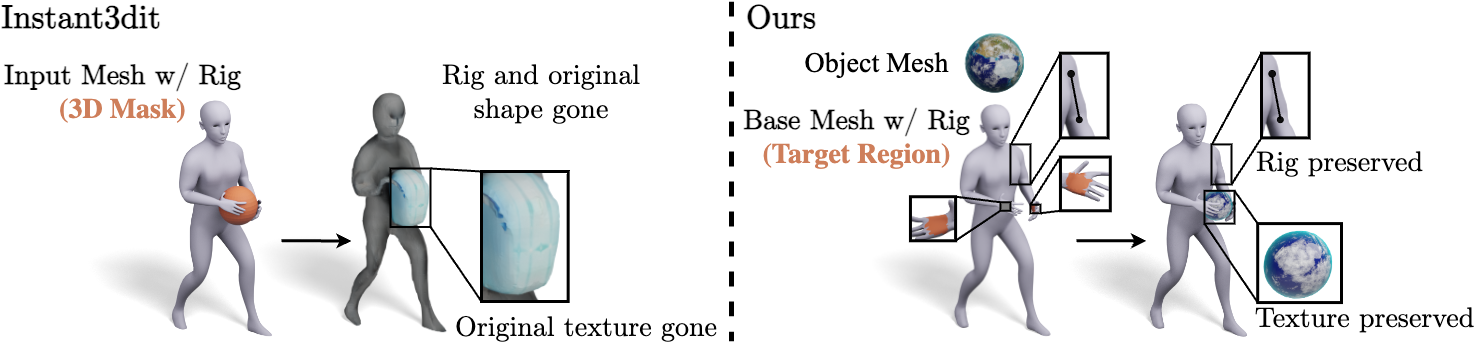
\includegraphics[width=\textwidth]{figures/instant3dit_comparison/instant3dit_comparison.png}
    \captionof{figure}{Digital artists often load shapes from pre-existing libraries of meshes that include additional information like animation rigs, skinning weights, texture maps and more. Generative shape editing methods like Instant3dit \cite{barda2025instant3dit} discard this information, performing global changes to the shapes and merging them together. \ourmethod{} is designed to fit exactly within this common artistic pipeline, and perfectly preserves all pre-existing information on the input meshes.}
    \label{fig:instant3dit_comparison}
    \vspace{-5.9mm}
\end{figure*}%


% Unfortunately, ...
However, recent advances in 3D content creation have focused mostly on \emph{generative} tasks; for example, creating shapes from text inputs~\cite{lin2023magic3d}.
These methods produce doubtlessly impressive results; yet, they do so at the cost of artist control and by relying on implicit geometric representations (e.g., radiance fields~\cite{mildenhall2021nerf} or Gaussian splats~\cite{kerbl20233d}) that are not directly usable in graphics pipelines.
Even when triangle meshes are generated~\cite{hao2024meshtron}, these are significantly lower in quality than those already available to artists in pre-existing shape libraries, lacking critical attributes like textures, animation rigs, and distinct material parameters. 







% We propose...
We propose \ourmethod{}, an optimization framework that progressively rotates, translates and then deforms an accessory until it fits tightly onto a base mesh while maximizing geometric, physical and semantic alignment.
We model this task's complexity by combining geometric losses based on distance between the meshes with physical losses preventing intersections and diffusion-based semantic guidance, and
devise a unique, multi-step optimization strategy in which each individual loss is introduced sequentially.

To succesfully navigate the ambiguities of the composition problem, we first assume that some coarse segmentation of the local ``fit'' region is highlighted, and use Vision-to-Language Model~\cite{gemini} agents to ensure adequate initialization. 
From this semantically-guided initial configuration, our algorithm drives the accessory closer to the base mesh, while using a GPU-optimized Bounding Volume Hierarchy to efficiently enforce non-intersection.
Similarly to how an artist may refine a pre-modeled accessory after optimizing its coarse position, our method optimizes a final deformation of the object through its Jacobians~\cite{aigerman2022neural}, maintaining physical realism by accounting for its (given or inferred) material parameters.










In this paper, we present a geometric optimization framework for reliably composing 3D meshes with accessories.
Through qualitative and quantitative comparisons, we show that our geometric optimization outperforms more general generative and 3D registration approaches for the task of mesh composition, while remaining intersection-free.
We show the robustness and applicability of our method on a diverse set of base meshes and accessories inspired by 3D content generation pipelines.